\linespread{1.5}
%use \usepackage{float}
\textbf{Solução}

\textbf{a)} O período da função é $T = 2\pi$, já que $f(t) = f(t+2\pi)$

\textbf{b)} 

\begin{figure}[H]
    \centering
    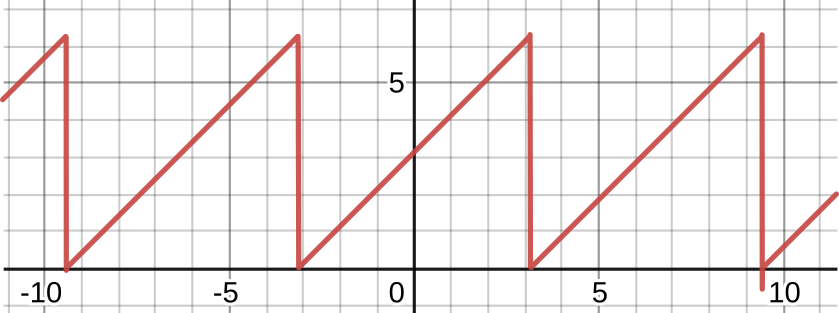
\includegraphics[width = 0.7\linewidth]{fig/sf6b.png}
    \caption{Como foi feita pelo site \textit{https://www.desmos.com/calculator} foi necessário limitar a série, o que permite ver os efeitos causados pela aproximação da série. Além disso no seu desenho deve mostrar os pontos que pertencem ou não aquela parte do gráfico, por exemplo: $-\pi \in y=0$, mas não pertence a $y=2\pi$, os saltos de uma função pra outra também não existem de fato na função.}
\end{figure}

\textbf{c)}
Nós podemos escrever a função \begin{equation}
    \label{eq:sf6cf}
    f(t) = f_1(t) + f_2(t) 
\end{equation} onde $f_1(t) = t$ e $f_2(t) = \pi$. 
Como $f_1(t) = t$ é uma função ímpar, não é necessário que calculamos os coeficientes $a_k$.

\begin{equation*}
    b_k = \frac{1}{\pi}\int_{-\pi}^\pi t\sin{(kwt)}dt = \left[-\frac{t\cos{(kwt)}}{kw}\right]^\pi_{\pi} - \int_{-\pi}^\pi\frac{(-\cos{(kwt)})}{kw}dt
\end{equation*}
\begin{equation*}
    = \frac{1}{\pi}\left\{\left[-\frac{t\cos{(kwt)}}{kw}\right]^\pi_{-\pi} + \left[\frac{\sin{(kwt)}}{(kw)^2}\right]^\pi_{-\pi}\right\}
\end{equation*}
\begin{equation*}
    = \frac{1}{\pi}\left\{\left[\left(\frac{-\pi\cos{(kw\pi)}}{kw}\right) - \left(\frac{\pi\cos{(-kwt)}}{kw}\right)\right] + \left[\left(\frac{\sin{(kw\pi)}}{(kw)^2}\right)-\left(\frac{\sin{(-kw\pi)}}{(kw)^2}\right)\right] \right\}
\end{equation*}
\begin{equation*}
    = \frac{1}{\pi}\left(\frac{-2\pi\cos{(kwt)}}{kw} + \frac{2\sin{(kw\pi)}}{(kw)^2}\right)
\end{equation*}
Como $w = \frac{2\pi}{T} = \frac{2\pi}{2\pi} = 1$, então:
\begin{equation}
    b_k = \frac{1}{\pi}\left(\frac{-2\pi\cos{(k\pi)}}{k} + \frac{2\sin{(k\pi)}}{k^2}\right) = \frac{2\cos{(k\pi)}}{k} = \frac{-2(-1)^k}{k}
\end{equation}
Pois temos que $\sin{(k\pi)} = 0 \forall k \in \Z$, Além disso $\cos{(k\pi)} = 1$ para $k$ par e $\cos{(k\pi)} = -1$ para $k$ ímpar, e dessa forma podemos dizer que $\cos{(k\pi)} = (-1)^k \forall k \in \N$. Dessa forma:
\begin{equation}
    \label{eq:sf6cf1}
    f_1(t) = \sum^\infty_{k=1} \frac{-2(-1)^k}{k}\sin{(kt)}
\end{equation}

Como $f_2(t)=\pi$ é uma função constante teremos que determinar somente o coeficiente de Fourier $a_0$. Contudo $a_0$ representa a média do comportamento da função podemos facilitar nossa vida e dizer que:
\begin{equation*}
    a_0 = \pi
\end{equation*}
e portanto 
\begin{equation}
    \label{eq:sf6cf2}
    f_2 = \pi
\end{equation}

Assim substituímos \ref{eq:sf6cf1} e \ref{eq:sf6cf2} em \ref{eq:sf6cf} teremos que:
\begin{equation}
    \label{sf6c}
    f(t) = f_1(t) + f_2(t) = \boxed{\pi + \sum^\infty_{k=1} \frac{-2(-1)^k}{k}\sin{(kt)}}
\end{equation}